 
\section{Problem 1}
\label{part1}
\begin{verbatim}
 Create a blog-term matrix.  Start by grabbing 100 blogs; include:

http://f-measure.blogspot.com/
http://ws-dl.blogspot.com/

and grab 98 more as per the method shown in class.  Note that this
method randomly chooses blogs and each student will separately do
this process, so it is unlikely that these 98 blogs will be shared
among students.  In other words, no sharing of blog data.  Upload
to github your code for grabbing the blogs and provide a list of
blog URIs, both in the report and in github..

Use the blog title as the identifier for each blog (and row of the
matrix).  Use the terms from every item/title (RSS) or entry/title
(Atom) for the columns of the matrix.  The values are the frequency
of occurrence.  Essentially you are replicating the format of the
``blogdata.txt'' file included with the PCI book code.  Limit the
number of terms to the most ``popular'' (i.e., frequent) 500 terms,
this is *after* the criteria on p. 32 (slide 7) has been satisfied.
 
\end{verbatim}

\subsection{Solution}

\begin{enumerate}
\item My task was to create a blog matrix and for that first I need to get all the blog URIs. 
\item I appended each URI with ``/feeds/posts/default?alt=rss''. The code for doing this can be found in listing\ref{lst:q1-1}.
\item Sample list of blog URIs can be found in fig\ref{Samplelist1} and sample list of URIs after appending can be found in fig\ref{Samplelist2}.
\item Now I found the number of pages in each blog using the code in the listing\ref{lst:q1-2}. Sample list of the number of pages in each blog can be found in fig\ref{Samplelist3}.
\item Now In order to find the blog matrix I used ``generatefeedvector.py'' code from Programming Collective Intelligence text.
\item I used feedparser library in order to parse the URI. I have made modification to the code to limit the words count to 500.
\item Each row in the blog represents a blog with blogname and each column is a specific word. Every cell in the matrix represent the number of times a word in present in that particular blog.
\item Some URIs did not allow the feedparser to parse through them. So I added some other URIs to my list in order to get 100 URIs.
\item I have also used stopwords so that irrelevant data is not entered into the blog matrix.
\item In the blog matrix there are 100 rows(blogs) and 500 columns(words). 
\item The frequency of each word in indicated in each cell of the matrix.
\item Python code for generating the blog matrix can be found in the listing\ref{lst:q1-3}.
\item Sample blog matrix can be seen in the fig\ref{Samplelist4}.
\end{enumerate}
\newpage
\subsection{Code Listing}

\lstinputlisting[language=Python,breaklines = true,frame=single,caption={Python code for getting 100 unique blog URIs and atom URIs}, label=lst:q1-1,captionpos=b,numbers=left,showspaces=false,showstringspaces=false,basicstyle=\footnotesize]{get_blogs.py}
\newpage

\subsection{Code Listing}

\lstinputlisting[language=Python,breaklines = true,frame=single,caption={Python code to find the number of pages in each blog}, label=lst:q1-2,captionpos=b,numbers=left,showspaces=false,showstringspaces=false,basicstyle=\footnotesize]{noOfPages.py}
\newpage

\subsection{Code Listing}

\lstinputlisting[language=Python,breaklines = true,frame=single,caption={Python code for getting blog matrix }, label=lst:q1-3,captionpos=b,numbers=left,showspaces=false,showstringspaces=false,basicstyle=\footnotesize]{generatefeedvector.py}
\newpage

\subsection{Outputs}

\subsubsection{Sample Blog URIs}
\begin{figure}[ht]    
    \begin{center}
        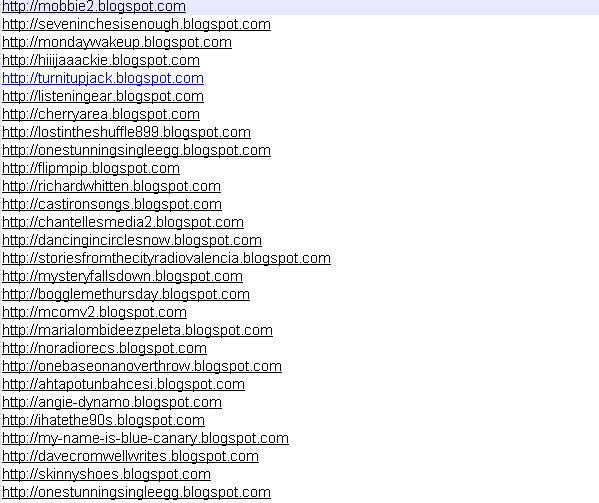
\includegraphics[scale=0.9]{sampleblogurls.png}
        \caption{Sample list of Blog URIs}
        \label{Samplelist1}
    \end{center}
\end{figure}
\newpage
\subsubsection{Sample atom URIs}
\begin{figure}[ht]    
    \begin{center}
        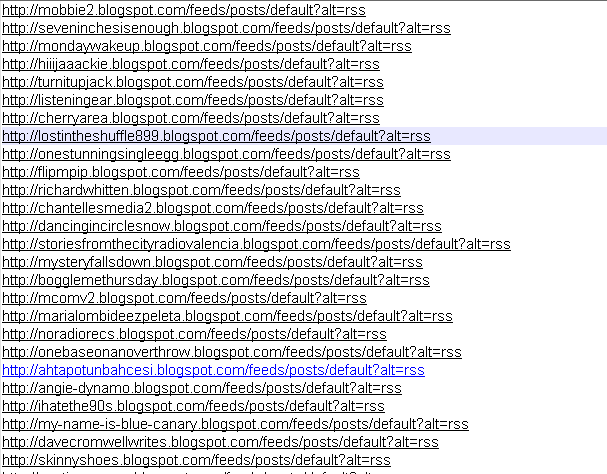
\includegraphics[scale=1.1]{sampleatomurls.png}
        \caption{Sample list of Atom URIs}
        \label{Samplelist2}
    \end{center}
\end{figure}
\newpage

\subsubsection{Sample number of pages}
\begin{figure}[ht]    
    \begin{center}
        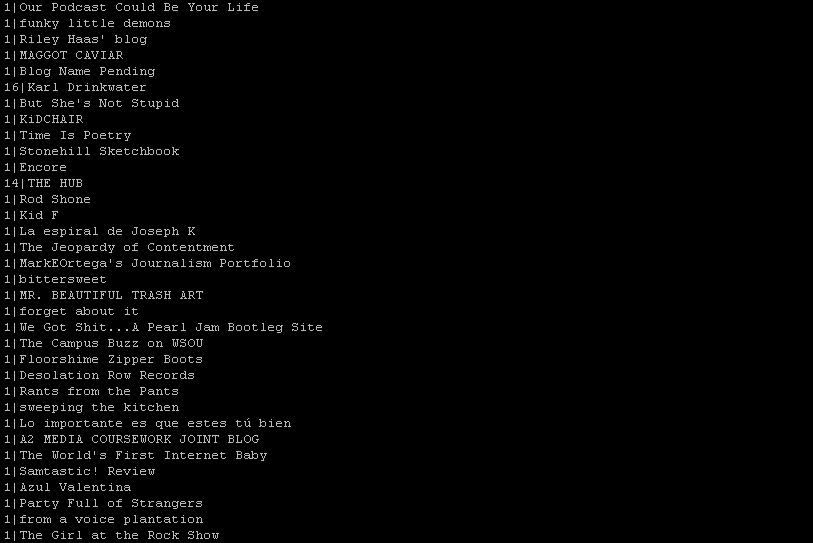
\includegraphics[scale=1.1]{samplenoofpages.png}
        \caption{Sample list of the number of pages in each blog}
        \label{Samplelist3}
    \end{center}
\end{figure}
\newpage

\subsubsection{Sample Blog matrix}
\begin{figure}[ht]    
    \begin{center}
        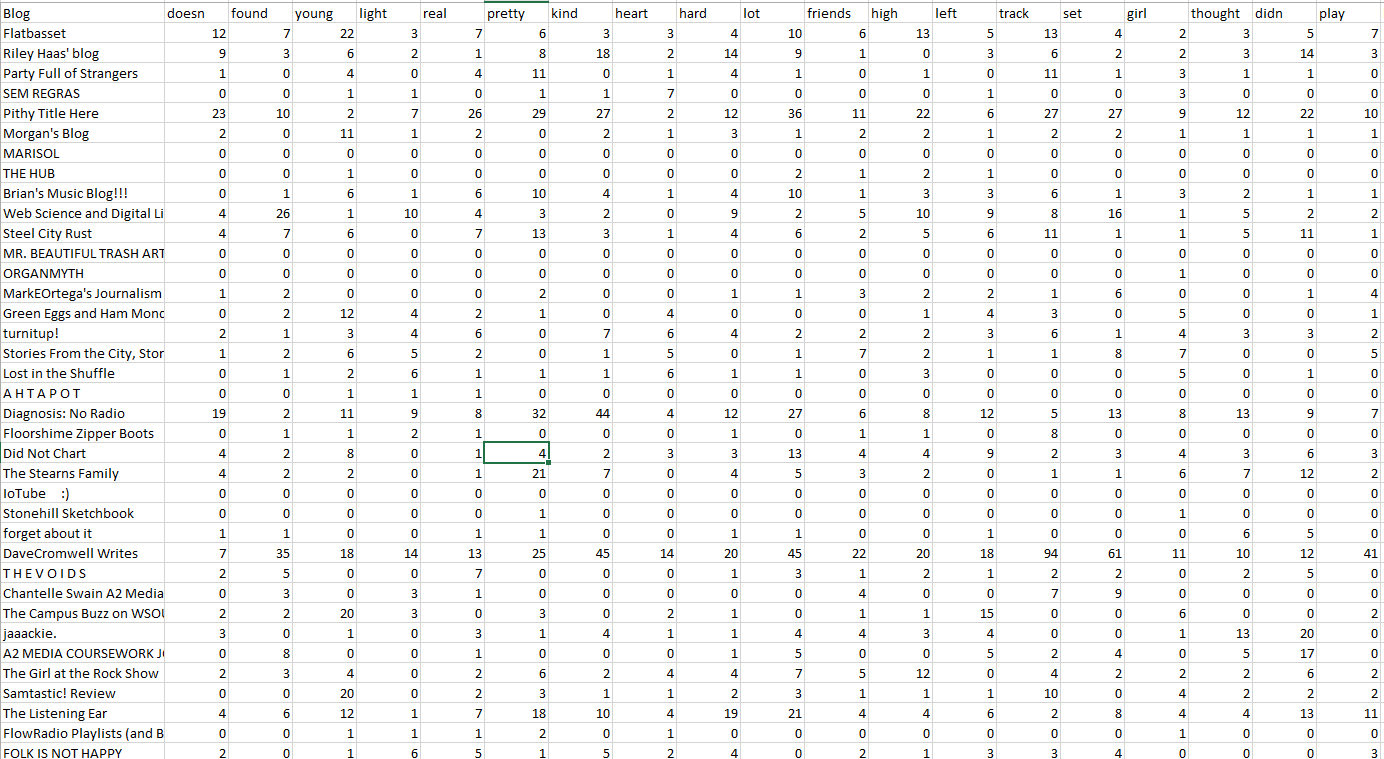
\includegraphics[scale=0.32]{sample_blogdata.png}
        \caption{Sample blogdata file}
        \label{q}
    \end{center}
\end{figure}
\newpage

